%%%%%%%%%%%%%%%%%%%%%%%%%%%%%%%%%%%%%%%%%%%%%%%%%%%
%
%  New template code for TAMU Theses and Dissertations starting Fall 2016.  
%
%
%  Author: Sean Zachary Roberson
%  Version 3.17.09
%  Last Updated: 9/21/2017
%
%%%%%%%%%%%%%%%%%%%%%%%%%%%%%%%%%%%%%%%%%%%%%%%%%%%

%%%%%%%%%%%%%%%%%%%%%%%%%%%%%%%%%%%%%%%%%%%%%%%%%%%%%%%%%%%%%%%%%%%%%%%
%%%                           SECTION II
%%%%%%%%%%%%%%%%%%%%%%%%%%%%%%%%%%%%%%%%%%%%%%%%%%%%%%%%%%%%%%%%%%%%%%

\chapter{\uppercase {Methodology}}

\section{The Acoustic Wave Equation}
I  assume an acoustic medium whose domain is $ \Omega \subset R^2$, and whose  boundary is $ \partial \Omega$  with  outward normal vector $\hat{n}$. The medium presents an acoustic velocity $c$ in $ \Omega$ and velocity  $c_b$ on  $ \partial  \Omega$. I want to find the transient propagation of pressure $p$ within the time interval $I=(0,T]$ produced  by a localized and known force $f$, where both $p$ and $f$ are functions of position $x \in \Omega$ and time $t \in I$, and in general $c$  is a function of position $x \in  \Omega$. I formulate the  PDE  for the acoustic wave propagation with absorbing boundary conditions as follows:
\begin{equation} \label{Eq2.1}
\begin{split}
 &\frac {\partial ^2 p} {\partial t^2}  - \nabla . \left(  c^2 \nabla p  \right)  = f   \quad  \textrm{in} \quad \Omega \times I, \\
 &\nabla p . \hat{n} = - \frac{1}{c_b} \frac{\partial p}{\partial t} \quad  \textrm{on} \quad \partial \Omega \times I,\\
 &p = 0  \quad \textrm{for} \quad t=0  \quad \textrm{in}  \quad \Omega, \\
 &\frac{\partial p}{\partial t} = 0 \quad \textrm{for} \quad t=0  \quad \textrm{in} \quad \Omega.
 \end{split}
\end{equation}

 I introduce the following change of variables $ v=\frac{\partial p}{\partial t}$ and  reformulate equation  \ref{Eq2.1}  as :
 \begin{equation} \label{Eq2.2}
 \begin{split}
  &v -\frac{\partial p}{\partial t} =0 \quad  \textrm{in} \quad \Omega \times I, \\
  &\frac{\partial v}{\partial t} - \nabla . \left(  c^2 \nabla p  \right)  = f   \quad  \textrm{in} \quad \Omega \times I, \\
  &\nabla p . \hat{n} = - \frac{1}{c_b}  \frac{\partial p}{\partial t} \quad  \textrm{on} \quad \partial \Omega \times I,\\
  &p = 0  \quad \textrm{for} \quad t=0  \quad \textrm{in}  \quad \Omega, \\
  & v= 0 \quad \textrm{for} \quad t=0  \quad \textrm{in} \quad \Omega.
  \end{split}
 \end{equation}
 
 The advantage of equation \ref{Eq2.2} is that it  only contains first order derivatives in time, which facilitates the use of  time  discretization schemes. 
 
\section{Weak Formulation of the Acoustic Wave Equation}
To obtain the weak form of equation \ref{Eq2.2}, I  take the inner product $(g_i,\phi)_D = \int_D g_i \phi$ between each element $g_i$ of the equation and a a test function $\phi \in  H^1(\Omega)$,  where  $H^1$ is a Hilbert space with at most  first derivatives in the distributional sense \cite{Brenner2008}, I also apply Gauss' theorem when necessary. Then, I formulate the weak form as follows:

Find $p$ and $v$  $\in  H^1(\Omega)$ such that:
 \begin{equation} \label{Eq2.3}
 \begin{split}
   & \left( v, \phi \right)_\Omega - \left( \frac{\partial p}{\partial t}  \phi \right)_\Omega  =0 \\
   & \left( \frac{\partial v}{\partial t}, \phi \right)_\Omega  + \left(  c_b \frac{\partial p}{\partial t} , \phi  \right)_{\partial \Omega} +
   \left(  c^2 \nabla p, \nabla \phi  \right)_\Omega = \left( f, \phi \right)_\Omega  
 \end{split}
 \end{equation}

\section{Space Discretization of the Weak Formulation: Continuous Galerkin Approach}
The strategy I use to discretize equation \ref{Eq2.3} in space and time is the Rothe's method \cite{Rothe1930}. In this approach, at each time step, a discrete PDE problem in space is solved by applying the FEM technique. 

To discretize equation \ref{Eq2.3} in space, I define a mesh $\tau$ covering the domain $\Omega \subset R^2$ with quadrilateral elements $\kappa \in \tau$ and the associated finite dimensional space $V_h  \subset H^1$. I also introduce a test function $\phi_h \in  V_h$ and formulate the discrete problem in space as:

Find $p_h$ and $v_h \in V_h$ such that:
 \begin{equation} \label{Eq2.4}
 \begin{split}
   &\left( \frac{\partial p_h}{\partial t}  \phi_h \right)_\Omega - \left( v_h, \phi_h \right)_\Omega    =0,\\
   & \left( \frac{\partial v_h}{\partial t}, \phi_h \right)_\Omega  + \left(  c_b \frac{\partial p_h}{\partial t} , \phi_h  \right)_{\partial \Omega} +
   \left(  c^2 \nabla p_h, \nabla \phi_h  \right)_\Omega = \left( f, \phi_h \right)_\Omega . 
 \end{split}
 \end{equation}
 
\subsection{The Standard FEM Approximation}
In general, the classical FEM incorporates piecewise polynomial basis functions $N_i (x) \in V_h$ to approximate the solution. Thus, I express the solution $p_h$ and $v_h$ as a linear combination of the basis functions $N_i(x)$:
 \begin{equation} \label{Eq2.5}
 \begin{split}
   & p_h=\sum_{i \in I}  P_i N_i(x),\\
   & v_h=\sum_{i \in I} B_i N_i(x).
 \end{split}
 \end{equation}

where $P_i$ and $B_i$ are the standard degrees of freedom (DOF) associated with the shape functions $N_i(x)$ and $I$ is the set of all nodes of DOF on the mesh $\tau$. For this work I restrict the basis functions to bilinear polynomials. 

\subsection{The GFEM Approximation}
This approximation technique exploits the partition of unity property of the standard FEM basis functions \cite{BABUSKA1997}:
 \begin{equation} \label{Eq2.6}
  \sum_{i \in I}  N_i(x)=1.\\
 \end{equation}

This property allows to reproduce any user-defined function $\psi_j(x)$ when multiplied by the partition of unity functions. Then the additional (enriched) basis functions are defined as the product between the standard basis functions and the enrichments:  $N_i(x) \psi_j(x)$. In this case, the solution approximation has a standard and an enriched part as follows:
 \begin{equation} \label{Eq2.7}
 \begin{split}
   & p_h=\sum_{i \in I} P_i N_i(x)  + \sum_{i \in I} N_i(x)  \sum_{j \in S} Q_j^i \psi_j(x)    , \\
   & v_h=\sum_{i \in I}B_i N_i(x)  +  \sum_{i \in I} N_i(x) \sum_{j \in S} C_j^i \psi_j(x)  .
 \end{split}
 \end{equation}

Where $Q_j^i$ and $C_j^i$  are the DOFs associated with the enriched basis functions $N_i(x) \psi_j(x)$, and $S$ is the set of user-defined enrichment functions. Usually, the enrichment functions are taken from closed form solutions to improve the FEM approximation. I define the enrichment functions $\psi  (x)$ with $x \in R^2$ as plane waves that can take different directions according to the unit wave number vector $\hat {k}_j$ as in \cite{Strouboulis2006}:
 \begin{equation} \label{Eq2.8}
 \begin{split}
   & S= \text{span}\lbrace \psi_j (x) =\cos \left(k \hat {k}_j. x \right)   \rbrace , \\
   & \text{with} \quad \hat {k}_j = \cos \frac{2 \pi j}{q} \hat {x}_1 + \sin \frac{2 \pi j}{q} \hat{x}_2 \quad j=0,...,q-1
 \end{split}
 \end{equation}
 
Where $k$ is the wave number, $q$ is the total number of directions for the plane wave, and $ \hat{x}_1$ and $\hat{x}_2$ are the the basis vectors in $R^2$ Cartesian coordinates.
For this work, the wave number used to define the enrichments is the maximum wave number  among the different geological bodies  present in a medium.

\subsection{Local Mesh Refinement}
In general, I use conforming quadrilateral meshes in $R^2$; however when needed I apply local mesh refinement by locally subdividing the elements of a mesh.  This operation leads to non-conforming meshes with hanging nodes (Figure \ref{fig:2.1}), meaning that some vertices of the refined elements will lie on the edge of neighboring unrefined elements \cite{Solin2008}. The main issue with this refinement technique is that  produces a lack of solution continuity across the edge of hanging nodes.

To ensure the continuity of the solution approximation, I impose that the dominating shape functions correspond to the unrefined elements across the edge of hanging nodes. Thus, I constrain the  DOF  of the refined elements  by a set of linear relationships relating the constrained  DOF $Dn_i$  with the unconstrained  DOF $D_j$ \cite{Bangerth2009}:
 \begin{equation} \label{Eq2.9}
   Dn_i= \sum_{j \in  I_m}\alpha_{ij} D_j \quad  \forall i \in I_n
 \end{equation}

where $I_n$ is the subset of constrained DOF, $I_m$ is the subset of unconstrained DOF, and $\alpha_{ij}$ are weighting factors relating the \textit{i-th} constrained DOF with the \textit{j-th} unconstrained DOF.

\begin{figure}[h!]
 		\centering
		\begin{subfigure}{5 cm}
				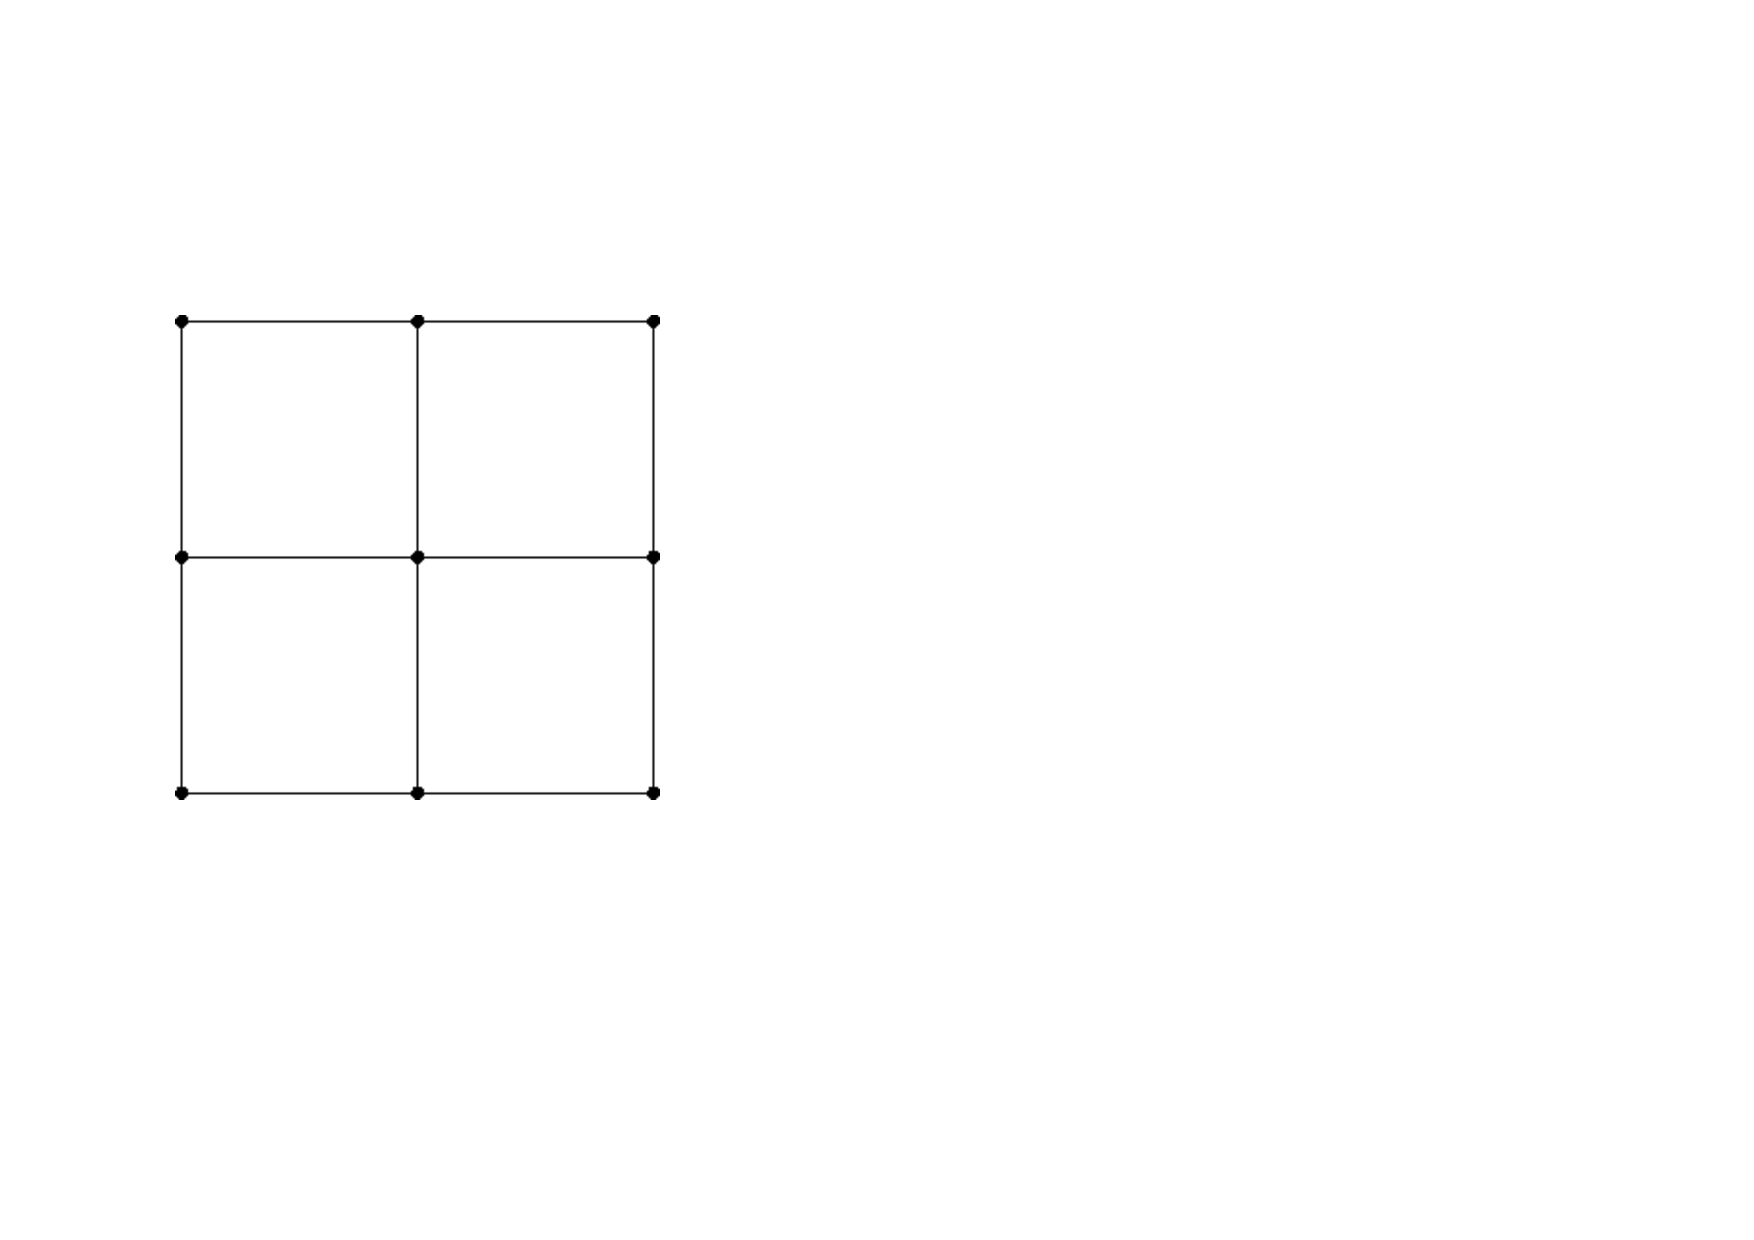
\includegraphics[width=5cm, height=5cm]{figures/coarse_mesh.pdf} 
			     \caption{}
				%\label{fig:trace1}
		\end{subfigure}
        \qquad
		\begin{subfigure}{10 cm}
				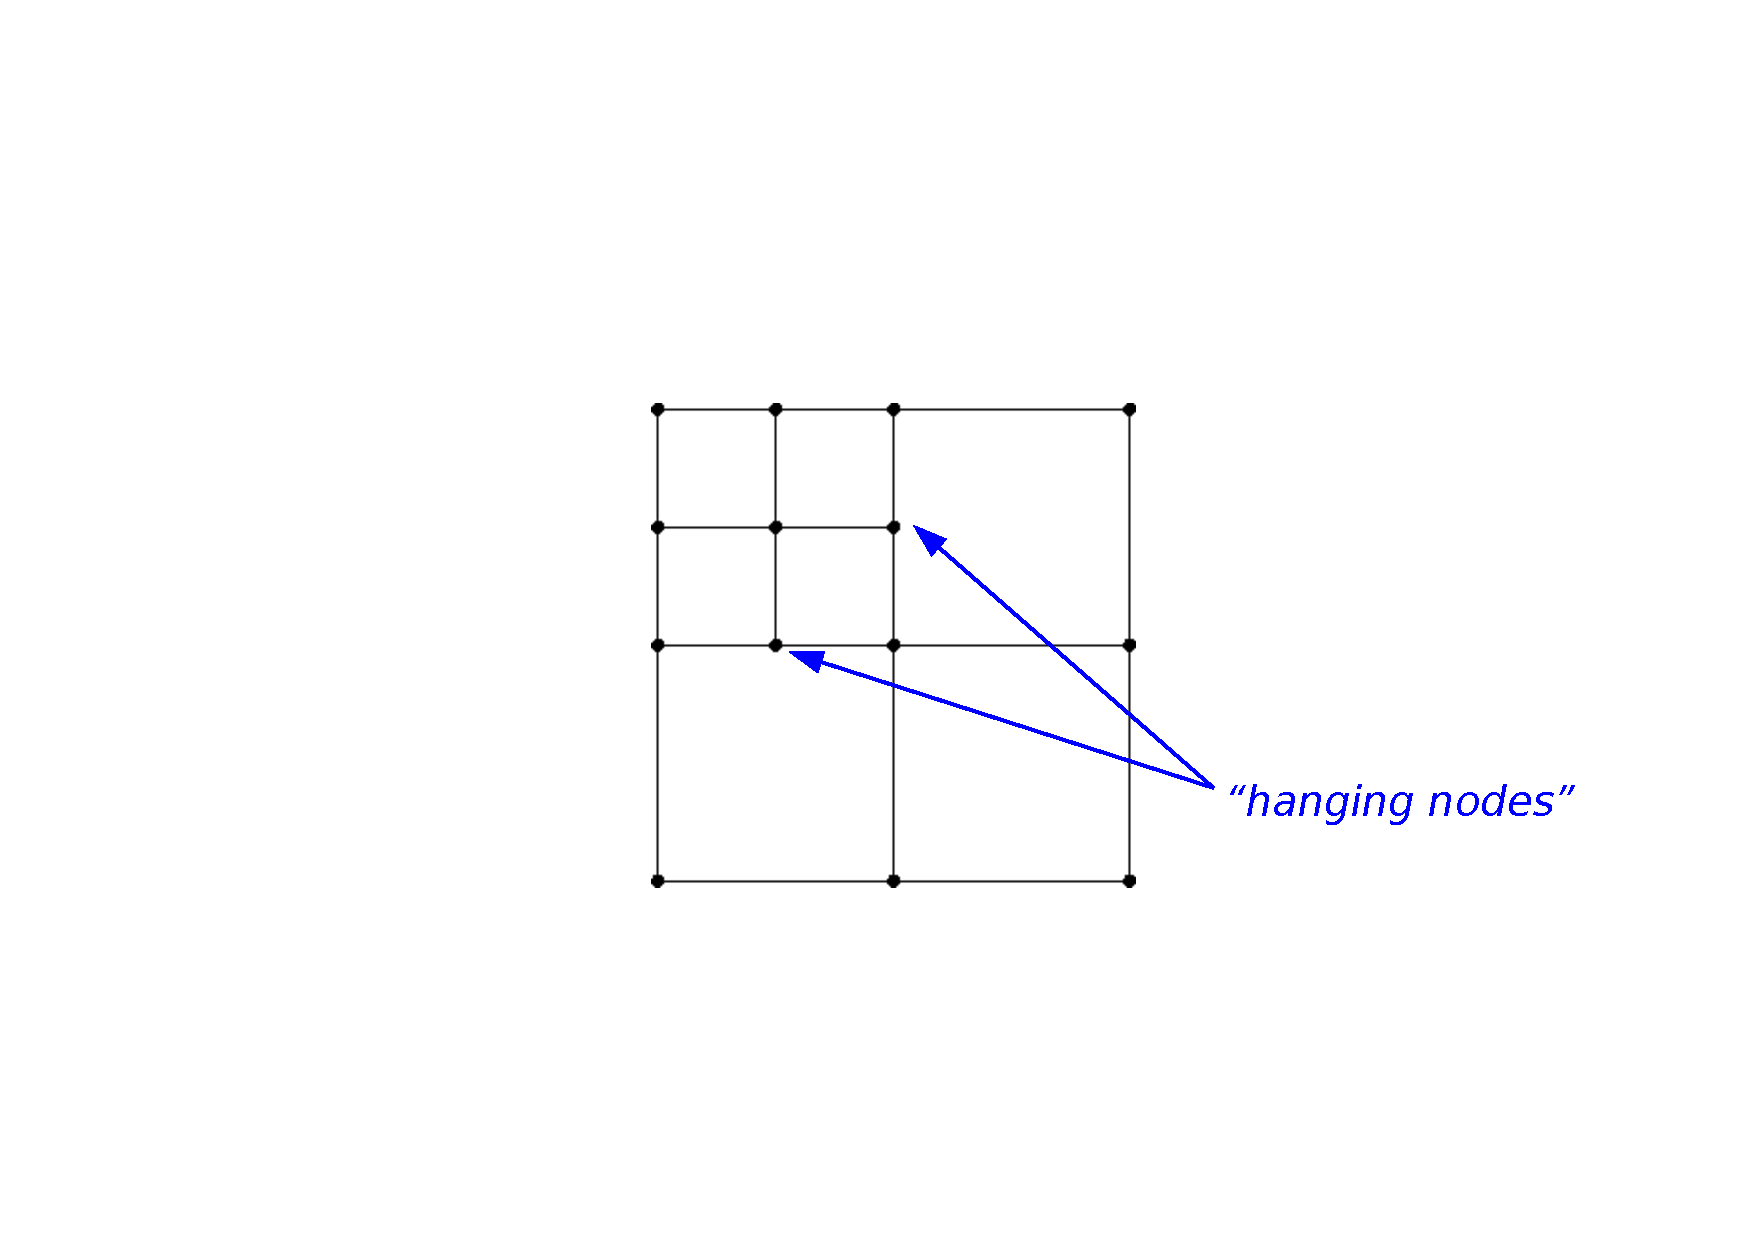
\includegraphics[width=9.2cm, height=5.3cm]{figures/mesh_hanging_nodes.pdf}
			   \caption{}
				%\label{fig:trace3}
		\end{subfigure}
 
	\caption{(a) Coarse Mesh. (b) Locally refined mesh with hanging nodes. Modified from class notes in \cite{Bangerth2013}. }
	\label{fig:2.1}
\end{figure}

\section{Time Discretization of the Weak Formulation}
For the time discretization, I subdivide  the time interval $I=(0,T]$ into sub-intervals $I_n=(t_{n-1}, t_n)$  of equal length $\Delta t =t_n-t_{n-1}$, where the discrete solution approximations for the corresponding times are $p_h^{n-1}$, $p_h^n$, and  $v_h^{n-1}$, $v_h^n$, respectively. Then, the time-discretized form of equation \ref{Eq2.4} applying the $\theta$-scheme with $\theta \in [0-1]$ is as follows:
 \begin{equation} \label{Eq2.10}
 \begin{split}
   & \left( p_h^n - p_h^{n-1},\phi_h \right)_\Omega -  \Delta t \left( \theta v_h^n + (1-\theta) v_h^{n-1}, \phi_h \right)_\Omega    =0,\\
   & \left( v_h^n-v_h^{n-1}, \phi_h \right)_\Omega  + \left(  c_b p_h^n - p_h^{n-1}, \phi_h  \right)_{\partial \Omega} + \Delta t \left( \theta c^2 \nabla p_h^n  + (1-\theta) c^2 \nabla p_h^{n-1}, \nabla \phi_h  \right)_\Omega\\
    &= \Delta t \left( \theta f^n +(1-\theta)f^{n-1}, \phi_h \right)_\Omega .
 \end{split}
 \end{equation}


\section{ Implementation}
For this work I  set $\theta =0.5$, for which the $ \theta$-method becomes the Crank-Nicholson scheme. Since I use the same mesh for every time step, the shape functions are the same for every time step as well: $\phi_h = \phi_h^n =\phi_h^{n-1} $. 
I also assume that solution vector is $D_p^n$  for $p_h$ and $D_v^n$ for $v_h$ at time $t_n$. The elements of these vectors are the DOF $D_{p_i}^n$  and $D_{v_i}^n$ at the nodes $i$. Then I can write the the solution approximation at the time step $t_n$ as:
 \begin{equation} \label{Eq2.11}
 \begin{split}
   & p_h^n=\sum_{i \in I}  D_{p_i}^n \phi_{h_i}(x),\\
   & v_h^n=\sum_{i \in I} D_{v_i}^n \phi_{h_i}(x).
 \end{split}
 \end{equation}
 
 Where, depending on the FEM approach, $\phi_{h_i}$ are either the standard FEM basis functions or the standard plus enriched basis functions. Thus, equation \ref{Eq2.11} is a generalization of equations \ref{Eq2.5} and \ref{Eq2.7}. Then, after replacing equation \ref{Eq2.11} into equation \ref{Eq2.10} and simplifying terms, I write equation \ref{Eq2.10} in matrix form as follows:
  \begin{equation} \label{Eq2.12}
 \begin{split}
   & L_p D_p^n = R_p, \\
   &L_v D_v^n = R_v.
 \end{split}
 \end{equation}
 
 Where matrices $L_p$ and  $L_v$ and vectors  $R_p$, and  $R_v$ are defined as follows:
 \begin{equation} \label{Eq2.13}
 \begin{split}
   &L_p = M + \Delta t \theta B +{\Delta t}^2 A, \\
   & L_v=M,\\
   &R_p= \left( M + \Delta t \theta B -{\Delta t}^2  \theta^2(1-\theta) A \right) D_p^{n-1}\\
   &+{\Delta t}^2  \theta^2 F^n + {\Delta t}^2 \theta F^{n-1},\\
   & R_v=M D_v^{n-1} + \left( B -  \Delta t (1-\theta) A \right) D_p^{n-1} \\
   & -\left(  B + \Delta t \theta A \right) D_p^n +\Delta t \theta F^n + \Delta t( 1- \theta) F^{n-1}.
 \end{split}
 \end{equation}
 
With matrices $M$, $A$ and $B$, and vectors $F^n$ and $F^{n-1}$ defined as:
 \begin{equation} \label{Eq2.14}
 \begin{split}
  & M_{ij}=(\phi_{h_i},\phi_{h_j})_\Omega,\\
  & A_{ij}=(c^2 \nabla \phi_{h_i},\nabla \phi_{h_j})_\Omega,\\
  & B_{ij} =(c_b  \phi_{h_i}, \phi_{h_j})_{\partial \Omega },\\
  & F_i^n = (f^n, \phi_{h_i})_\Omega,\\
  & F_i^{n-1} = (f^{n-1}, \phi_{h_i})_\Omega.\\
 \end{split}
 \end{equation}

I also define the continuous function $f (x,t)$ in a similar way as in \cite{Yue2005}:
 \begin{equation} \label{Eq2.15}
 \begin{split}
  & f(x,t) = a_o f_1(t) f_2(x),\\
  &  f_1(t) = f_o (t-t_o) \exp \left( \pi^2 f_o^2 (t-t_o)^2   \right) \quad \forall \quad t \leq t_o,\\
  & f_2(x) =\left( 1- \frac{\Vert x - r_o \Vert ^2 }{R_s^2} \right)^3 \frac{1}{V} \quad \forall \quad \Vert x-r_o \Vert \leq R_s, \\ 
  & V =\frac{\pi}{4} R_s^2.\\
 \end{split}
 \end{equation}

Where $f(x,t) =f$ is the right hand side of the PDE defined in equation \ref{Eq2.1} and represents a seismic source,  $a_o$ is a scaling factor, $f_o = 1/t_o$ is the central frequency of the source, $r_o$ is the source center, $\Vert .\Vert$ is the Euclidean distance and $R_s$ is the source radius. The spatial part of the source $f_2(x)$ is normalized by its volume $V$, so that the size of the source does not affect the wave amplitude, at least from a theoretical point of view. In a numerical implementation, however, source size might have an effect on the wave amplitude when the mesh size is not fine enough to sample the source a required number of times. I explore the source size effect in the GFEM simulations in section 3.1.1.

\subsection{Mesh Generation and Numerical Simulation}
All the software I use for this work is open source. I use \textbf{gmsh} \cite{Geuzaine2009} to generate quadrilateral meshes. The advantage of \textbf{gmsh} is that it allows for flexible meshing, generating elements that conform to complex geometry boundaries. It also has the capability to control element size in different regions of the mesh, keeping mesh regularity. I also use \textbf{tethex} (https://github.com/martemyev/tethex/wiki), which is a utility that arranges \textbf{gmsh} mesh output to a format that is compatible with the FEM library \textbf{deal.II} \cite{Bangerth2007} that I use to implement the acoustic wave simulation. \textbf{deal.II}  provides the necessary tools  for simulation with FEM, including classes that implement the standard and enriched  basis functions \cite{Davydov2017}. This library is built using object-oriented programming in C++, with modular classes that include mesh generation, definition of finite element spaces, linear solvers and post-processing capabilities among others. \textbf{deal.II} can create non-conforming locally refined meshes and has the capability to handle hanging node constraints to maintain  the continuity of  the finite element space . Although for this work I implement a continuous Galerkin formulation, \textbf{deal.II} also allows for a discontinuous Galerkin implementation.
\textbf{deal.II} implements finite element linear systems, as the ones in equation \ref{Eq2.12}, in the standard fashion, by performing calculations at each element $K$ of a mesh $\tau$. For instance:  $(.,.)_\Omega= \displaystyle\sum_{K \in \tau} (.,.)_K$.

\section{Error Estimate}
%revise this
The proposed method estimates the error between the traces obtained  using the GFEM and a reference solution, in which the reference solution results from applying the FEM in a fine mesh. For that I define an error measure $E_k$:

 \begin{equation} \label{Eq2.17}
  E_k =\left| 1 - \left|  \frac{ CC_k }{AC_0 }  \right| \right|
 \end{equation}

Where $CC_k$ is the cross correlation between the test and reference solution either for the zero lag ($k=0$) or at the maximum cross correlation value ($k=max$) and $AC_0$ is the zero lag auto correlation of the reference solution.
